\documentclass[25pt, a0paper, portrait]{tikzposter}
\tikzposterlatexaffectionproofoff %% remove the mark on the bottom right

\usepackage{hyperref}
\usepackage{booktabs}
\usepackage{adjustbox}
\usepackage{multicol}
\usepackage{listings}
\usepackage{stmaryrd, amssymb}


\definecolor{Black}{RGB}{0,0,0}

\RequirePackage[T1]{fontenc}
\RequirePackage{fontspec}
\fontspec[AutoFakeBold=3.5]{IMFellEnglish-Regular.ttf}

%% Font of the text, might use a different one for the title
%% that matches better the New York Times front page.
\setmainfont{IMFellEnglish}[
  Path=./,
  Extension = .ttf,
  UprightFont = *-Regular,
  ItalicFont = *-Italic,
  BoldFont= *-Regular,
  BoldFeatures={FakeBold=3.5},
]

%% Custom background and frame, we only need it to be white
\definebackgroundstyle{samplebackgroundstyle}{
  \draw[inner sep=0pt, line width=0pt, color=white, fill=white]
  (bottomleft) rectangle (topright);
}

%% Custom title, nothing really, just remove the ugly frame
\definetitlestyle{sampletitlestyle}{
  width=500mm, roundedcorners=20, linewidth=2pt, innersep=5pt,
  titletotopverticalspace=15mm, titletoblockverticalspace=30mm
}{}

%% Custom block style, we want a title and that's it.
\defineblockstyle{sampleblockstyle}{
    titlewidthscale=1, bodywidthscale=1, titleleft,
    titleoffsetx=0pt, titleoffsety=0pt, bodyoffsetx=0pt, bodyoffsety=0pt,
    bodyverticalshift=0pt, roundedcorners=0,
    titleinnersep=0.5cm, bodyinnersep=0.5cm
}{ %% nothing really
}

%% Colors
\definecolorstyle{samplecolorstyle} {
  \definecolor{colorOne}{named}{yellow}
  \definecolor{colorTwo}{named}{black}
  \definecolor{colorThree}{named}{cyan}
} {
  \colorlet{backgroundcolor}{colorOne}
  \colorlet{framecolor}{black}
  \colorlet{blocktitlefgcolor}{black}
  \colorlet{blocktitlebgcolor}{white}
}

\definelayouttheme{sample}{
  \usecolorstyle{samplecolorstyle}
  \usetitlestyle{sampletitlestyle}
  \usebackgroundstyle{samplebackgroundstyle}
  \useblockstyle{sampleblockstyle}
  \useinnerblockstyle{sampleblockstyle}
}

\usetheme{sample}


\makeatletter
\renewcommand\Huge{\@setfontsize\Huge{135}{135}}
\renewcommand\huge{\@setfontsize\Huge{120}{120}}
\renewcommand\LARGE{\@setfontsize\Huge{70}{70}}
\renewcommand\Large{\@setfontsize\Huge{60}{60}}
\renewcommand\large{\@setfontsize\Huge{50}{50}}
\renewcommand\normalsize{\@setfontsize\Huge{40}{40}} %% between 24-36
\renewcommand\small{\@setfontsize\Huge{20}{20}}
\renewcommand\footnotesize{\@setfontsize\Huge{15}{15}}
\renewcommand\scriptsize{\@setfontsize\Huge{12}{12}}
\renewcommand\tiny{\@setfontsize\Huge{10}{10}} 
\makeatother

\newcommand{\TOPBLOCK}{0.17}

\settitle{
  \centering
  \begin{tabular}{p{\TOPBLOCK\columnwidth}p{0.62\columnwidth}p{\TOPBLOCK\columnwidth}}
    \adjustbox{max width=\TOPBLOCK\columnwidth}{\fbox{\parbox{\dimexpr\linewidth-2\fboxsep-2\fboxrule}
        {``\@author ~ from \textit{\@institute}''}}} &
    \centering\bfseries\Huge\@title &
    \adjustbox{max width=\TOPBLOCK\columnwidth}{{\parbox{\dimexpr\linewidth-2\fboxsep-2\fboxrule}{
          \begin{center}
            \textbf{ISWC edition}
          \end{center}
          
          The 22$^{nd}$ International Semantic Web Conference: The
          premier international forum for the Semantic Web and Linked
          Data Community.}}} \vspace{0.25em}\\ \midrule
    
    & \centering\textsc{\uppercase{Athens, Greece, 6-10 November 2023}} & \hfill\$0.00\\ \bottomrule
  \end{tabular}
}

\newcommand{\HRULE}{\centerline{\rule{0.6667\linewidth}{0.1cm}}}



\title{RAW-JENA}

\author{Julien Aimonier-Davat, Minh-Hoang Dang, Pascal Molli, Brice Nédelec, and Hala Skaf-Molli}
\date{November 6--10}
\institute{Nantes Université, CNRS, LS2N}

\setlength{\columnsep}{1.5cm}

\begin{document}
\maketitle[width=\columnwidth]

\begin{columns}
  \column{0.74}
  \block{\huge Approximate Query Processing for SPARQL Endpoints}{
    \begin{multicols}{2}
      \begin{center}
        \HRULE
        \textit{Integrate sampling as SQL did with the TABLESAMPLE clause.}
        \HRULE
      \end{center}
      
      Sample-based approximate query processing (S-AQP) has many
      important use cases for RDF such as computing
      \begin{itemize}
      \item large-scale statistics,
      \item knowledge graph embeddings,
      \item join orders,
      \item approximate aggregations,
      \item summaries,
      \item exploratory queries.
      \end{itemize}
      \ \\
      By confining query execution to samples of large datasets,
      S-AQP drastically
      \begin{itemize}
      \item reduces execution time, 
      \item delivering approximate results
      \item with error estimates.
      \end{itemize}
    \end{multicols}%
  }
  \draw[line width=0.2cm] (blocktitle.north east) -- (blockbody.south east);%
  %
  \column{0.26}
  \block{Ad-hoc sampling}{
    \begin{center}
      \HRULE
      \textit{is not great!}
      \HRULE
      
      \uppercase{May time out on public SPARQL endpoints\ldots}
      \HRULE
    \end{center}
    
    \texttt{SELECT * \{?s ?p ?o\} OFFSET r LIMIT 1}, where $r$ is a
    random number between 0 and the dataset size (0 $< r <$ 12B).\\

    %% Well-known engines such as
    %% Stardog\footnote{\url{https://docs.stardog.com/query-stardog/sampling-service\#sampling-service}},
    %% or
    %% Virtuoso\footnote{https://docs.openlinksw.com/virtuoso/rndsalltr/},
    %% propose an ad-hoc sampling API, but with no guarantee on complexity.\\
  }
\end{columns}

\block{Random walks for cardinality estimates and confidence with WanderJoin}{
  \fbox{
    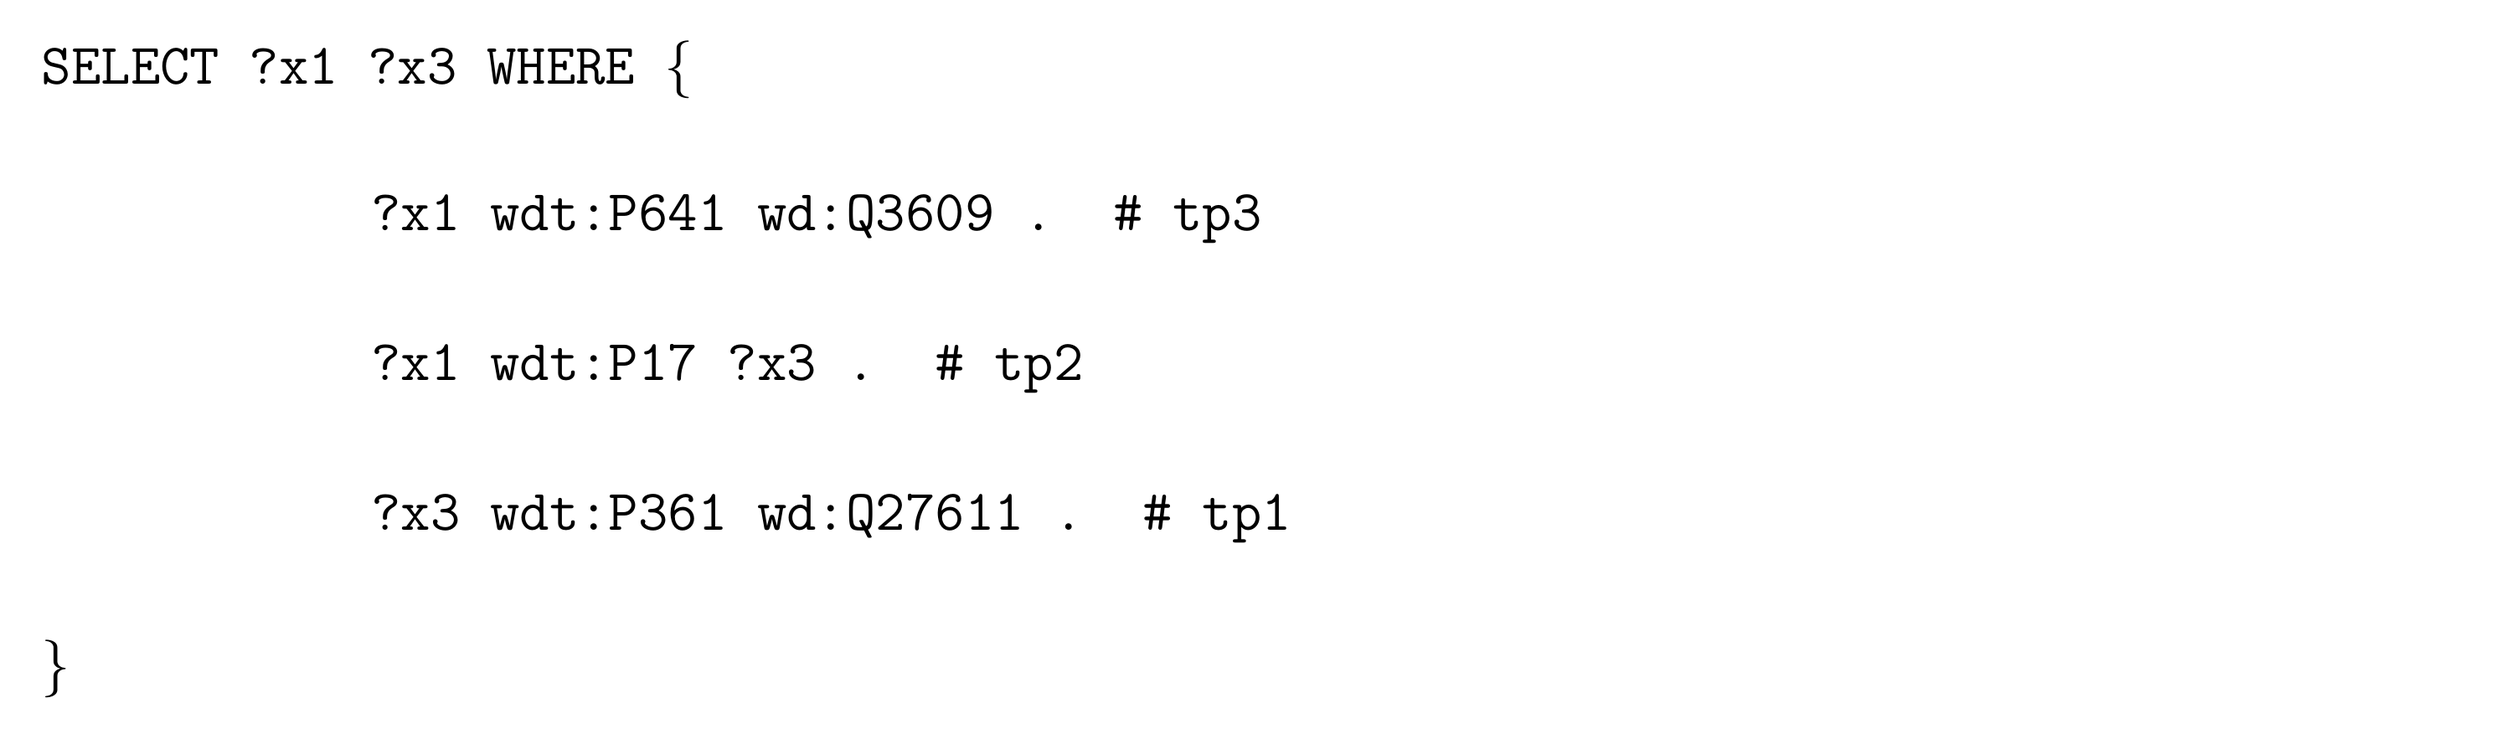
\begin{tikzpicture}
      \newcommand\X{5cm}
      \newcommand\Y{-2.273cm}
      \draw[anchor=west] (0*\X,0*\Y) node {\texttt{SELECT ?x1 ?x3 WHERE \{}};
      \draw[anchor=west] (1*\X,1*\Y) node {\texttt{?x1 wdt:P641 wd:Q3609  .         \# tp3}};
      \draw[anchor=west] (1*\X,2*\Y) node {\texttt{?x1 wdt:P17  ?x3       .         \# tp2}};
      \draw[anchor=west] (1*\X,3*\Y) node {\texttt{?x3 wdt:P361 wd:Q27611 .         \# tp1}};
      \draw[anchor=west] (0*\X,4*\Y) node {\texttt{\}}};
      \draw (7*\X,0*\Y) node {\hphantom{positioning}};
    \end{tikzpicture}
  }
  \fbox{
    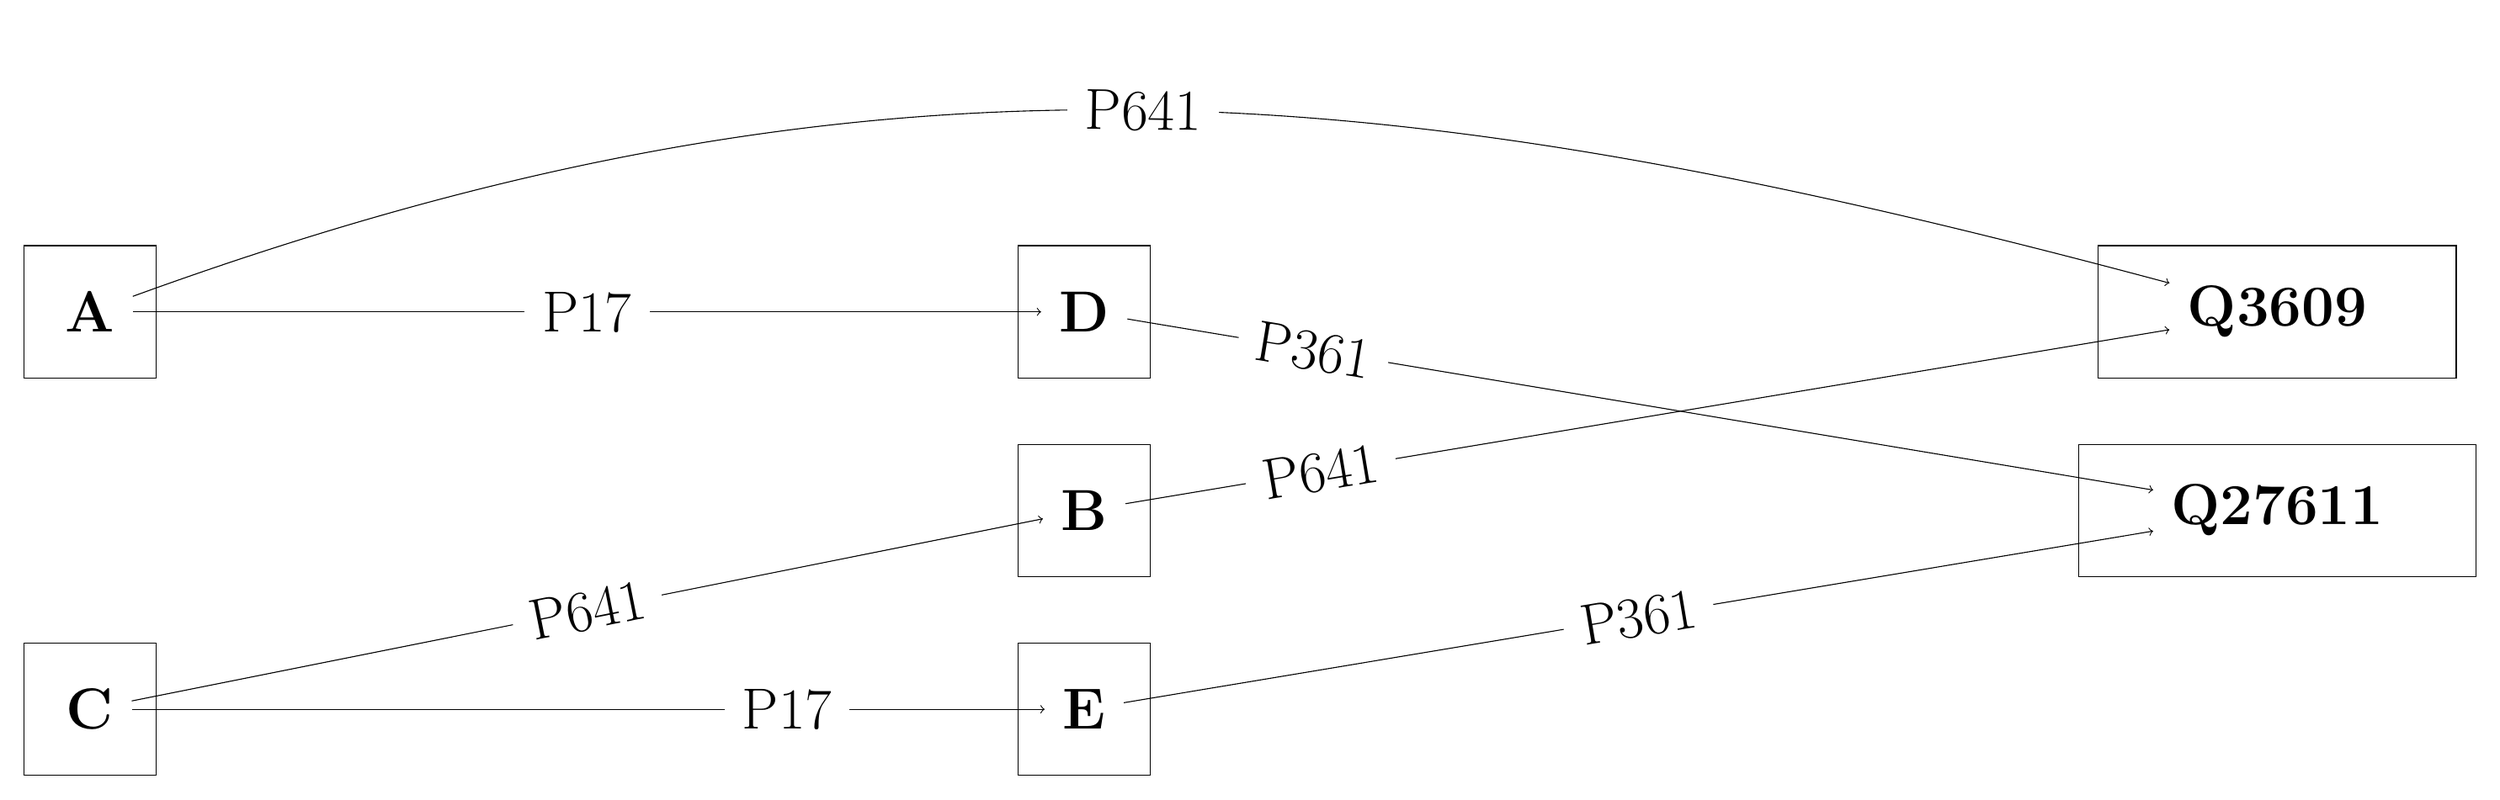
\begin{tikzpicture}
      \thickmuskip=0mu
      \medmuskip=0mu
      \thinmuskip=0mu
      
      \newcommand\X{15cm}
      \newcommand\Y{-3cm}
      \newcommand\PREDICATE{\normalsize}
      \newcommand{\RECTSIZE}{1cm}
      
      \draw (0, 0) node(A){\textbf{A}} +(-\RECTSIZE, -\RECTSIZE) rectangle +(\RECTSIZE, \RECTSIZE);
      \draw (\X, 0) node(D){\textbf{D}} +(-\RECTSIZE, -\RECTSIZE) rectangle +(\RECTSIZE, \RECTSIZE);
      \draw (2.2*\X, 0) node(Q3609){\textbf{Q3609}} +(-2.7*\RECTSIZE, -\RECTSIZE) rectangle +(2.7*\RECTSIZE, \RECTSIZE);
      
      \draw (\X, \Y) node(B){\textbf{B}} +(-\RECTSIZE, -\RECTSIZE) rectangle +(\RECTSIZE, \RECTSIZE);
      \draw (2.2*\X, \Y) node(Q27611){\textbf{Q27611}} +(-3*\RECTSIZE, -\RECTSIZE) rectangle +(3*\RECTSIZE, \RECTSIZE);
      \draw (0, 2*\Y) node(C){\textbf{C}} +(-\RECTSIZE, -\RECTSIZE) rectangle +(\RECTSIZE, \RECTSIZE);
      \draw (1*\X, 2*\Y) node(E){\textbf{E}} +(-\RECTSIZE, -\RECTSIZE) rectangle +(\RECTSIZE, \RECTSIZE);
      

      \draw[->] (A) -- node[fill=white, font=\PREDICATE]{P17} (D);
      \draw[->] (C) -- node[fill=white, sloped, font=\PREDICATE]{P641} (B);
      \draw[->] (C) -- node[fill=white, sloped, font=\PREDICATE, xshift=3cm]{P17} (E);
      \draw[->] (B) -- node[fill=white, sloped, font=\PREDICATE, xshift=-5cm]{P641} (Q3609);
      \draw[->] (E) -- node[fill=white, sloped, font=\PREDICATE]{P361} (Q27611);
      \draw[->] (D) -- node[fill=white, sloped, font=\PREDICATE, xshift=-5cm]{P361} (Q27611);
      \draw[->] (A) to[out=20, in=165] node[fill=white,sloped, font=\PREDICATE]{P641} (Q3609);
      
    \end{tikzpicture}
    }\\
  %
  \adjustbox{max width=0.4\columnwidth}{Figure 1: Query $Q_1$: All cycling races of Central America along with their respective country.}
  \hspace{7cm}
  \adjustbox{max width=0.45\columnwidth}{Figure 2: RDF Graph $G_1$: $A$, $B$, and $C$ are cycling sports; $D$ and $E$ are countries of Central
    America.}\\

  % Let $Q$ be a SPARQL conjunctive query, and $J = \langle tp_1, ..., tp_n \rangle$ be
  % the join order to perform random walks. A random walk
  % $\gamma_i = \langle t_1, ..., t_n\rangle$ is computed over
  % an RDF graph $G$ by randomly picking $t_1$ in $\llbracket tp_1 \rrbracket_G$,
  % and each subsequent $t_i$ ($i > 1$) in $\llbracket t_{i-1} \bowtie tp_i \rrbracket_G$.
  % Once computed, the cardinality of $Q$ is estimated as  the inverse probability
  % of sampling $\gamma_i$~\cite{li2019wanderjoin}, with

  $P(\gamma_i) = |\llbracket tp_1 \rrbracket_G|^{-1} \prod_{i=2}^{n}
  |\llbracket t_{i-1} \bowtie tp_i \rrbracket_G|^{-1}$.

  %% For instance, let us consider the query $Q_1$ and the RDF graph $G_1$
  %% depicted in Figure~\ref{fig:random_walks_example}. Following the join order $tp_3,tp_2,tp_1$, the random walk $\gamma_1$ is computed as
  %% follows:

\begin{center}
  \begin{tabular}{l|lll}
    $tp_3$ & draw  $t_1$ &$= (\textbf{A}, P641, Q3609)$ & $\in \llbracket (?x1, P641, Q3609) \rrbracket_{G_1}$ \\
    $tp_2$ & draw  $t_2$ &$= (A, P17, \textbf{D})$ & $ \in \llbracket (\textbf{A}, P17, ?x3) \rrbracket_{G_1}$  \\
    $tp_1$ & draw  $t_3$ &$= (D, P361, Q27611)$ & $\in \llbracket (\textbf{D}, P361, Q27611) \rrbracket_{G_1}$  
  \end{tabular}
\end{center} 

%% \noindent The cardinality of $Q_1$ is then estimated as the inverse
%% probability of sampling $\gamma_1$:

\begin{small}
$P(\gamma_1)^{-1}  =  |\llbracket (?x1, P641, Q3609) \rrbracket_{G_1}| \cdot
                          |\llbracket (\textbf{A}, P17, ?x3) \rrbracket_{G_1}| \cdot
                          |\llbracket (\textbf{D}, P361,
                          Q27611) \rrbracket_{G_1}| 
                      =  2 \cdot 1 \cdot 1 = 2$
\end{small}

%% \begin{small}
%% \begin{tabular}{ll}
%%     $P(\gamma_1)^{-1}$  &$=  |\llbracket (?x1, P641, Q3609) \rrbracket_{G_1}| \times
%%                           |\llbracket (\textbf{A}, P17, ?x3) \rrbracket_{G_1}| \times
%%                           |\llbracket (\textbf{D}, P361,
%%                           Q27611) \rrbracket_{G_1}| $ \\
%%                       &$=  2 \times 1 \times 1 = 2$
%% \end{tabular}
%% \end{small}

\noindent Note that a random walk may fail if it becomes impossible to sample $t_i$ for
some $i \leq n$. In this case, its probability $P(\gamma_i)$ of being sampled is 0.
For instance, if $t_1 = (B, P641, Q3609)$ is picked in
$\llbracket (?x1, P641, Q3609) \rrbracket_{G_1}$
instead of $(A, P641, Q3609)$, then the random walk fails because
$\llbracket (B, P17, ?x3) \rrbracket_{G_1} = \varnothing$.
%
To improve the quality of estimates, we compute a set of $k$ random
walks $\Gamma = \langle \gamma_1, ..., \gamma_k \rangle$, and the
cardinality of $Q$ is estimated as
\smash{$|\Gamma|^{-1}\sum_{i=1}^{|\Gamma|} P(\gamma_i)^{-1}$}.
  
}


\begin{columns} % See Section 4.4
  \column{0.33} % See Section 4.4
  \block{Conclusion}{
      In Apache Jena
      Modifying balanced trees\\
      Implementing cardinality estimation
      Rather simple
  }
  \column{0.33}
  \block{Perspective}{
    More operators
  }
  \column{0.33}
  \block{}{
    
\includegraphics[width=0.28\textwidth]{images/qr-code.png}
    \begin{center}
      \url{https://github.com/gdd-nantes/raw-jena}
    \end{center}
  }
\end{columns}

\block{References}{
  WanderJoin
  S-AQP
  virtuoso
  stardog
}

\end{document}
